% Created by tikzDevice version 0.12 on 2019-06-12 19:07:25
% !TEX encoding = UTF-8 Unicode
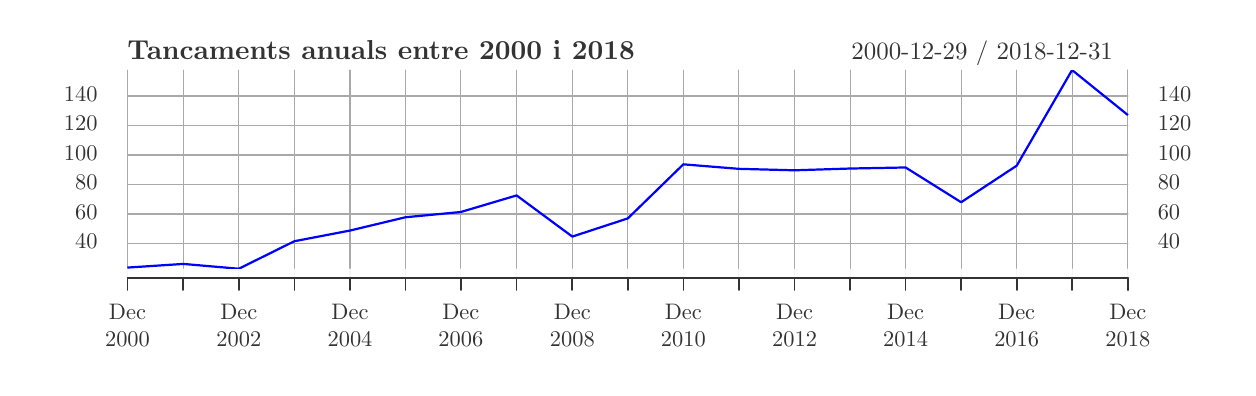
\begin{tikzpicture}[x=1pt,y=1pt]
\definecolor{fillColor}{RGB}{255,255,255}
\path[use as bounding box,fill=fillColor,fill opacity=0.00] (0,0) rectangle (433.62,122.86);
\begin{scope}
\path[clip] ( 21.60, 32.40) rectangle (412.02,122.86);
\definecolor{drawColor}{RGB}{169,169,169}

\path[draw=drawColor,line width= 0.4pt,line join=round,line cap=round] ( 36.06, 35.75) -- ( 36.06,107.54);

\path[draw=drawColor,line width= 0.4pt,line join=round,line cap=round] ( 56.23, 35.75) -- ( 56.23,107.54);

\path[draw=drawColor,line width= 0.4pt,line join=round,line cap=round] ( 76.30, 35.75) -- ( 76.30,107.54);

\path[draw=drawColor,line width= 0.4pt,line join=round,line cap=round] ( 96.36, 35.75) -- ( 96.36,107.54);

\path[draw=drawColor,line width= 0.4pt,line join=round,line cap=round] (116.48, 35.75) -- (116.48,107.54);

\path[draw=drawColor,line width= 0.4pt,line join=round,line cap=round] (136.49, 35.75) -- (136.49,107.54);

\path[draw=drawColor,line width= 0.4pt,line join=round,line cap=round] (156.51, 35.75) -- (156.51,107.54);

\path[draw=drawColor,line width= 0.4pt,line join=round,line cap=round] (176.68, 35.75) -- (176.68,107.54);

\path[draw=drawColor,line width= 0.4pt,line join=round,line cap=round] (196.80, 35.75) -- (196.80,107.54);

\path[draw=drawColor,line width= 0.4pt,line join=round,line cap=round] (216.86, 35.75) -- (216.86,107.54);

\path[draw=drawColor,line width= 0.4pt,line join=round,line cap=round] (236.93, 35.75) -- (236.93,107.54);

\path[draw=drawColor,line width= 0.4pt,line join=round,line cap=round] (256.94, 35.75) -- (256.94,107.54);

\path[draw=drawColor,line width= 0.4pt,line join=round,line cap=round] (277.11, 35.75) -- (277.11,107.54);

\path[draw=drawColor,line width= 0.4pt,line join=round,line cap=round] (297.18, 35.75) -- (297.18,107.54);

\path[draw=drawColor,line width= 0.4pt,line join=round,line cap=round] (317.24, 35.75) -- (317.24,107.54);

\path[draw=drawColor,line width= 0.4pt,line join=round,line cap=round] (337.31, 35.75) -- (337.31,107.54);

\path[draw=drawColor,line width= 0.4pt,line join=round,line cap=round] (357.38, 35.75) -- (357.38,107.54);

\path[draw=drawColor,line width= 0.4pt,line join=round,line cap=round] (377.39, 35.75) -- (377.39,107.54);

\path[draw=drawColor,line width= 0.4pt,line join=round,line cap=round] (397.56, 35.75) -- (397.56,107.54);

\path[draw=drawColor,line width= 0.4pt,line join=round,line cap=round] (397.56, 35.75) -- (397.56,107.54);
\end{scope}
\begin{scope}
\path[clip] (  0.00,  0.00) rectangle (433.62,122.86);
\definecolor{drawColor}{gray}{0.96}

\path[draw=drawColor,line width= 0.4pt,line join=round,line cap=round] ( 36.06, 32.40) -- (397.56, 32.40);

\path[draw=drawColor,line width= 0.4pt,line join=round,line cap=round] ( 36.06, 32.40) -- ( 36.06, 35.64);

\path[draw=drawColor,line width= 0.4pt,line join=round,line cap=round] ( 56.23, 32.40) -- ( 56.23, 35.64);

\path[draw=drawColor,line width= 0.4pt,line join=round,line cap=round] ( 76.30, 32.40) -- ( 76.30, 35.64);

\path[draw=drawColor,line width= 0.4pt,line join=round,line cap=round] ( 96.36, 32.40) -- ( 96.36, 35.64);

\path[draw=drawColor,line width= 0.4pt,line join=round,line cap=round] (116.48, 32.40) -- (116.48, 35.64);

\path[draw=drawColor,line width= 0.4pt,line join=round,line cap=round] (136.49, 32.40) -- (136.49, 35.64);

\path[draw=drawColor,line width= 0.4pt,line join=round,line cap=round] (156.51, 32.40) -- (156.51, 35.64);

\path[draw=drawColor,line width= 0.4pt,line join=round,line cap=round] (176.68, 32.40) -- (176.68, 35.64);

\path[draw=drawColor,line width= 0.4pt,line join=round,line cap=round] (196.80, 32.40) -- (196.80, 35.64);

\path[draw=drawColor,line width= 0.4pt,line join=round,line cap=round] (216.86, 32.40) -- (216.86, 35.64);

\path[draw=drawColor,line width= 0.4pt,line join=round,line cap=round] (236.93, 32.40) -- (236.93, 35.64);

\path[draw=drawColor,line width= 0.4pt,line join=round,line cap=round] (256.94, 32.40) -- (256.94, 35.64);

\path[draw=drawColor,line width= 0.4pt,line join=round,line cap=round] (277.11, 32.40) -- (277.11, 35.64);

\path[draw=drawColor,line width= 0.4pt,line join=round,line cap=round] (297.18, 32.40) -- (297.18, 35.64);

\path[draw=drawColor,line width= 0.4pt,line join=round,line cap=round] (317.24, 32.40) -- (317.24, 35.64);

\path[draw=drawColor,line width= 0.4pt,line join=round,line cap=round] (337.31, 32.40) -- (337.31, 35.64);

\path[draw=drawColor,line width= 0.4pt,line join=round,line cap=round] (357.38, 32.40) -- (357.38, 35.64);

\path[draw=drawColor,line width= 0.4pt,line join=round,line cap=round] (377.39, 32.40) -- (377.39, 35.64);

\path[draw=drawColor,line width= 0.4pt,line join=round,line cap=round] (397.56, 32.40) -- (397.56, 35.64);
\end{scope}
\begin{scope}
\path[clip] (  0.00,  0.00) rectangle (433.62,122.86);
\definecolor{drawColor}{gray}{0.20}

\path[draw=drawColor,line width= 0.4pt,line join=round,line cap=round] ( 36.06, 32.40) -- (397.56, 32.40);

\path[draw=drawColor,line width= 0.6pt,line join=round,line cap=round] ( 36.06, 32.40) -- ( 36.06, 28.08);

\path[draw=drawColor,line width= 0.6pt,line join=round,line cap=round] ( 56.23, 32.40) -- ( 56.23, 28.08);

\path[draw=drawColor,line width= 0.6pt,line join=round,line cap=round] ( 76.30, 32.40) -- ( 76.30, 28.08);

\path[draw=drawColor,line width= 0.6pt,line join=round,line cap=round] ( 96.36, 32.40) -- ( 96.36, 28.08);

\path[draw=drawColor,line width= 0.6pt,line join=round,line cap=round] (116.48, 32.40) -- (116.48, 28.08);

\path[draw=drawColor,line width= 0.6pt,line join=round,line cap=round] (136.49, 32.40) -- (136.49, 28.08);

\path[draw=drawColor,line width= 0.6pt,line join=round,line cap=round] (156.51, 32.40) -- (156.51, 28.08);

\path[draw=drawColor,line width= 0.6pt,line join=round,line cap=round] (176.68, 32.40) -- (176.68, 28.08);

\path[draw=drawColor,line width= 0.6pt,line join=round,line cap=round] (196.80, 32.40) -- (196.80, 28.08);

\path[draw=drawColor,line width= 0.6pt,line join=round,line cap=round] (216.86, 32.40) -- (216.86, 28.08);

\path[draw=drawColor,line width= 0.6pt,line join=round,line cap=round] (236.93, 32.40) -- (236.93, 28.08);

\path[draw=drawColor,line width= 0.6pt,line join=round,line cap=round] (256.94, 32.40) -- (256.94, 28.08);

\path[draw=drawColor,line width= 0.6pt,line join=round,line cap=round] (277.11, 32.40) -- (277.11, 28.08);

\path[draw=drawColor,line width= 0.6pt,line join=round,line cap=round] (297.18, 32.40) -- (297.18, 28.08);

\path[draw=drawColor,line width= 0.6pt,line join=round,line cap=round] (317.24, 32.40) -- (317.24, 28.08);

\path[draw=drawColor,line width= 0.6pt,line join=round,line cap=round] (337.31, 32.40) -- (337.31, 28.08);

\path[draw=drawColor,line width= 0.6pt,line join=round,line cap=round] (357.38, 32.40) -- (357.38, 28.08);

\path[draw=drawColor,line width= 0.6pt,line join=round,line cap=round] (377.39, 32.40) -- (377.39, 28.08);

\path[draw=drawColor,line width= 0.6pt,line join=round,line cap=round] (397.56, 32.40) -- (397.56, 28.08);

\path[draw=drawColor,line width= 0.6pt,line join=round,line cap=round] (397.56, 32.40) -- (397.56, 28.08);

\node[text=drawColor,anchor=base,inner sep=0pt, outer sep=0pt, scale=  0.81] at ( 36.06, 27.00) {};

\node[text=drawColor,anchor=base,inner sep=0pt, outer sep=0pt, scale=  0.81] at ( 36.06, 17.28) {Dec};

\node[text=drawColor,anchor=base,inner sep=0pt, outer sep=0pt, scale=  0.81] at ( 36.06,  7.56) {2000};

\node[text=drawColor,anchor=base,inner sep=0pt, outer sep=0pt, scale=  0.81] at ( 76.30, 27.00) {};

\node[text=drawColor,anchor=base,inner sep=0pt, outer sep=0pt, scale=  0.81] at ( 76.30, 17.28) {Dec};

\node[text=drawColor,anchor=base,inner sep=0pt, outer sep=0pt, scale=  0.81] at ( 76.30,  7.56) {2002};

\node[text=drawColor,anchor=base,inner sep=0pt, outer sep=0pt, scale=  0.81] at (116.48, 27.00) {};

\node[text=drawColor,anchor=base,inner sep=0pt, outer sep=0pt, scale=  0.81] at (116.48, 17.28) {Dec};

\node[text=drawColor,anchor=base,inner sep=0pt, outer sep=0pt, scale=  0.81] at (116.48,  7.56) {2004};

\node[text=drawColor,anchor=base,inner sep=0pt, outer sep=0pt, scale=  0.81] at (156.51, 27.00) {};

\node[text=drawColor,anchor=base,inner sep=0pt, outer sep=0pt, scale=  0.81] at (156.51, 17.28) {Dec};

\node[text=drawColor,anchor=base,inner sep=0pt, outer sep=0pt, scale=  0.81] at (156.51,  7.56) {2006};

\node[text=drawColor,anchor=base,inner sep=0pt, outer sep=0pt, scale=  0.81] at (196.80, 27.00) {};

\node[text=drawColor,anchor=base,inner sep=0pt, outer sep=0pt, scale=  0.81] at (196.80, 17.28) {Dec};

\node[text=drawColor,anchor=base,inner sep=0pt, outer sep=0pt, scale=  0.81] at (196.80,  7.56) {2008};

\node[text=drawColor,anchor=base,inner sep=0pt, outer sep=0pt, scale=  0.81] at (236.93, 27.00) {};

\node[text=drawColor,anchor=base,inner sep=0pt, outer sep=0pt, scale=  0.81] at (236.93, 17.28) {Dec};

\node[text=drawColor,anchor=base,inner sep=0pt, outer sep=0pt, scale=  0.81] at (236.93,  7.56) {2010};

\node[text=drawColor,anchor=base,inner sep=0pt, outer sep=0pt, scale=  0.81] at (277.11, 27.00) {};

\node[text=drawColor,anchor=base,inner sep=0pt, outer sep=0pt, scale=  0.81] at (277.11, 17.28) {Dec};

\node[text=drawColor,anchor=base,inner sep=0pt, outer sep=0pt, scale=  0.81] at (277.11,  7.56) {2012};

\node[text=drawColor,anchor=base,inner sep=0pt, outer sep=0pt, scale=  0.81] at (317.24, 27.00) {};

\node[text=drawColor,anchor=base,inner sep=0pt, outer sep=0pt, scale=  0.81] at (317.24, 17.28) {Dec};

\node[text=drawColor,anchor=base,inner sep=0pt, outer sep=0pt, scale=  0.81] at (317.24,  7.56) {2014};

\node[text=drawColor,anchor=base,inner sep=0pt, outer sep=0pt, scale=  0.81] at (357.38, 27.00) {};

\node[text=drawColor,anchor=base,inner sep=0pt, outer sep=0pt, scale=  0.81] at (357.38, 17.28) {Dec};

\node[text=drawColor,anchor=base,inner sep=0pt, outer sep=0pt, scale=  0.81] at (357.38,  7.56) {2016};

\node[text=drawColor,anchor=base,inner sep=0pt, outer sep=0pt, scale=  0.81] at (397.56, 27.00) {};

\node[text=drawColor,anchor=base,inner sep=0pt, outer sep=0pt, scale=  0.81] at (397.56, 17.28) {Dec};

\node[text=drawColor,anchor=base,inner sep=0pt, outer sep=0pt, scale=  0.81] at (397.56,  7.56) {2018};
\end{scope}
\begin{scope}
\path[clip] ( 21.60,107.54) rectangle (412.02,119.51);
\definecolor{drawColor}{gray}{0.20}

\node[text=drawColor,anchor=base west,inner sep=0pt, outer sep=0pt, scale=  0.99] at ( 36.06,111.25) {\bfseries Tancaments anuals entre 2000 i 2018};

\node[text=drawColor,anchor=base east,inner sep=0pt, outer sep=0pt, scale=  0.90] at (392.16,111.46) {2000-12-29 / 2018-12-31};
\end{scope}
\begin{scope}
\path[clip] ( 21.60, 35.75) rectangle (412.02,107.54);
\definecolor{drawColor}{RGB}{169,169,169}

\path[draw=drawColor,line width= 0.4pt,line join=round,line cap=round] ( 36.06, 44.88) -- (397.56, 44.88);

\path[draw=drawColor,line width= 0.4pt,line join=round,line cap=round] ( 36.06, 55.54) -- (397.56, 55.54);

\path[draw=drawColor,line width= 0.4pt,line join=round,line cap=round] ( 36.06, 66.20) -- (397.56, 66.20);

\path[draw=drawColor,line width= 0.4pt,line join=round,line cap=round] ( 36.06, 76.86) -- (397.56, 76.86);

\path[draw=drawColor,line width= 0.4pt,line join=round,line cap=round] ( 36.06, 87.52) -- (397.56, 87.52);

\path[draw=drawColor,line width= 0.4pt,line join=round,line cap=round] ( 36.06, 98.17) -- (397.56, 98.17);
\end{scope}
\begin{scope}
\path[clip] (  0.00,  0.00) rectangle (433.62,122.86);
\definecolor{drawColor}{gray}{0.20}

\node[text=drawColor,anchor=base east,inner sep=0pt, outer sep=0pt, scale=  0.81] at ( 25.26, 43.02) { 40};

\node[text=drawColor,anchor=base east,inner sep=0pt, outer sep=0pt, scale=  0.81] at ( 25.26, 53.68) { 60};

\node[text=drawColor,anchor=base east,inner sep=0pt, outer sep=0pt, scale=  0.81] at ( 25.26, 64.34) { 80};

\node[text=drawColor,anchor=base east,inner sep=0pt, outer sep=0pt, scale=  0.81] at ( 25.26, 75.00) {100};

\node[text=drawColor,anchor=base east,inner sep=0pt, outer sep=0pt, scale=  0.81] at ( 25.26, 85.66) {120};

\node[text=drawColor,anchor=base east,inner sep=0pt, outer sep=0pt, scale=  0.81] at ( 25.26, 96.32) {140};

\node[text=drawColor,anchor=base west,inner sep=0pt, outer sep=0pt, scale=  0.81] at (408.36, 43.02) { 40};

\node[text=drawColor,anchor=base west,inner sep=0pt, outer sep=0pt, scale=  0.81] at (408.36, 53.68) { 60};

\node[text=drawColor,anchor=base west,inner sep=0pt, outer sep=0pt, scale=  0.81] at (408.36, 64.34) { 80};

\node[text=drawColor,anchor=base west,inner sep=0pt, outer sep=0pt, scale=  0.81] at (408.36, 75.00) {100};

\node[text=drawColor,anchor=base west,inner sep=0pt, outer sep=0pt, scale=  0.81] at (408.36, 85.66) {120};

\node[text=drawColor,anchor=base west,inner sep=0pt, outer sep=0pt, scale=  0.81] at (408.36, 96.32) {140};
\end{scope}
\begin{scope}
\path[clip] ( 21.60, 35.75) rectangle (412.02,107.54);
\definecolor{drawColor}{RGB}{0,0,255}

\path[draw=drawColor,line width= 0.8pt,line join=round] ( 36.06, 36.17) --
	( 56.23, 37.49) --
	( 76.30, 35.75) --
	( 96.36, 45.69) --
	(116.48, 49.55) --
	(136.49, 54.35) --
	(156.51, 56.25) --
	(176.68, 62.24) --
	(196.80, 47.37) --
	(216.86, 53.94) --
	(236.93, 73.48) --
	(256.94, 71.85) --
	(277.11, 71.32) --
	(297.18, 71.96) --
	(317.24, 72.34) --
	(337.31, 59.78) --
	(357.38, 72.99) --
	(377.39,107.54) --
	(397.56, 91.28);
\end{scope}
\end{tikzpicture}
